%%%%%%%%%%%%%%%%%%%%%%%%%%%%%%%%%%%%%%%%%%%%%%%%%%%%%%%%%%%%%%%%%%%%%%%%%%%%%%%%
%% 서울대학교 데이터마이닝연구실 구성원들의 박사학위논문 작성을 위해 아래 저작자의 자료를 일부 수정하였습니다.
%% Author: zeta709 (zeta709@gmail.com) 
%%%%%%%%%%%%%%%%%%%%%%%%%%%%%%%%%%%%%%%%%%%%%%%%%%%%%%%%%%%%%%%%%%%%%%%%%%%%%%%%
%% 2018-01-08 산업공학과 데이터마이닝 전공을 산업공학과로 수정하고, 영어 석사 논문 작성 시 편리한 작업을 위한 추가 수정 및 팁 작성 by 문지형 jhmoon@dm.snu.ac.kr

\RequirePackage{fix-cm} 
% oneside : 단면 인쇄용
% twoside : 양면 인쇄용
% ms: 석
% phd : 박사
% openright : 챕터가 홀수쪽에서 시작
\documentclass[oneside,ms]{snuthesis_utf8}

%%%%%%%%%%%%%%%%%%%%%%%%%%%%%%%%%%%%%%%%
%% 목차 양식을 변경하는 코드
%% subfigure (subfig) package 사용 여부에 따라
%% tocloft의 옵션을 다르게 지정해야 한다.
%\usepackage[titles,subfigure]{tocloft} % when you use subfigure package
\usepackage[titles]{tocloft} % when you don't use subfigure package
\makeatletter % don't delete me
\renewcommand\cftchappresnum{Chapter~}
\renewcommand\cftfigpresnum{Figure~}
\renewcommand\cfttabpresnum{Table~}


\usepackage[pdftex,bookmarks=true]{hyperref}
\usepackage{tabularx}
\usepackage{array,multirow,graphicx,rotating,booktabs}
\usepackage{caption}  %subfigure
\usepackage{subcaption}  %subfigure
\usepackage[round, sort, numbers]{natbib} %reference style
\newcommand\mycite[1]{[\citenum{#1}]}
\newcommand\myauthor[1]{\citeauthor{#1} (\citeyear{#1})}
\usepackage{pbox} % line break in table
\usepackage{adjustbox}
\usepackage{footnote}
\usepackage{color,soul}
\usepackage{colortbl}
\usepackage{amsmath}
\usepackage{float} % position here
\usepackage{lscape} % for landscape page
\usepackage{kotex}
\usepackage{listings}

\makeatother % don't delete me
\newlength{\mytmplen}
\settowidth{\mytmplen}{\bfseries\cftchappresnum\cftchapaftersnum}
\addtolength{\cftchapnumwidth}{\mytmplen}
\settowidth{\mytmplen}{\bfseries\cftfigpresnum\cftfigaftersnum}
\addtolength{\cftfignumwidth}{\mytmplen}
\settowidth{\mytmplen}{\bfseries\cfttabpresnum\cfttabaftersnum}
\addtolength{\cfttabnumwidth}{\mytmplen}
%% 목차 양식을 변경하는 코드 끝
%%%%%%%%%%%%%%%%%%%%%%%%%%%%%%%%%%%%%%%%

%%%%%%%%%%%%%%%%%%%%%%%%%%%%%%%%%%%%%%%%
%% 다른 패키지 로드
%% http://faq.ktug.or.kr/faq/pdflatex%B0%FAlatex%B5%BF%BD%C3%BB%E7%BF%EB
%% 필요에 따라 직접 수정 필요
\ifpdf
	% \input glyphtounicode\pdfgentounicode=1 %type 1 font사용시
	%\usepackage[pdftex,unicode]{hyperref} % delete me
	%\usepackage[pdftex]{graphicx}
	%\usepackage[pdftex,svgnames]{xcolor}
\else
	%\usepackage[dvipdfmx,unicode]{hyperref} % delete me%
	%\usepackage[dvipdfmx]{graphicx}
	%\usepackage[dvipdfmx,svgnames]{xcolor}
\fi
%%%%%%%%%%%%%%%%%%%%%%%%%%%%%%%%%%%%%%%%
%
%% \title : 22pt로 나오는 큰 제목
%% \title* : 16pt로 나오는 작은 제목
\title{Practical Partial Row Activation\\ for 3D Stacked DRAM with Applications to Deep Learning Workloads}
\title*{3D 적층 DRAM을 위한 실용적인 Partial Row Activation 및 딥 러닝 워크로드에의 적용}

\titlen{Practical Partial Row Activation\\ for 3D Stacked DRAM with Applications to Deep Learning Workloads}

\author{Namho~Kim}
\author*{Namho~Kim} % Same as \author.
\authorn{Namho~Kim}
\phonenumber{010-5120-5105}
\studentnumber{2017-22393}
\advisor{Jae~W.~Lee}
\advisor*{Jae W. Lee}
\advisorn{Jae~W.~Lee}
\graddate{February~2019}
\submissiondate{January~2019}
\submissiondaten{January~20th,~2019}
\approvaldate{January~2019}

\committeemembers%
{Jihong Kim}%
{Jae W. Lee}%
{Jaejin Lee}%
{교 수 님}%
{교 수 님} %

%% Length of underline
\setlength{\committeenameunderlinelength}{5cm}

\begin{document}
\pagenumbering{Roman}
\makefrontcover
\makeapproval

%agreement page
\cleardoublepage
%\makeagreement

\cleardoublepage
\pagenumbering{roman}

\keyword{DRAM Architecture, GPU, Convolutional Neural Network, HBM2, Power Efficiency}
\begin{abstract}
GPUs are widely used to run deep learning applications. 
Today's high-end GPUs adopt 3D stacked DRAM technologies like High-Bandwidth Memory (HBM) to provide massive bandwidth, which consumes lots of power. 
Thousands of concurrent threads on GPU cause frequent row buffer conflicts to waste a significant amount of DRAM energy. 
To reduce this waste we propose a \emph{practical} partial row activation scheme for 3D stacked DRAM. 
Exploiting the latency tolerance of deep learning workloads with abundant memory-level parallelism, we trade DRAM latency for energy savings. 
The proposed design demonstrates substantial savings of DRAM activation energy with minimal performance degradation for both the deep learning and other conventional GPU workloads. 
This benefit comes with a very low area cost and only minimal adjustments of DRAM timing parameters to the standard HBM2 DRAM interface.
\end{abstract}
\cleardoublepage

% % 여기 수정할 것
\tableofcontents
\addcontentsline{toc}{chapter}{\contentsname}
\cleardoublepage

\listoftables
\addcontentsline{loc}{chapter}{\listtablename}
\cleardoublepage

\listoffigures
\addcontentsline{loc}{chapter}{\listfigurename}
\cleardoublepage

\pagenumbering{arabic}

\chapter{Introduction}
The recent advent of throughput computing with Graphics Processing Units (GPU) led an increase in demand for the memory bandwidth. To meet this increasing demand for memory bandwidth, 3D-stacked memory technologies such as High-Bandwidth Memory (HBM) \mycite{HBMstandard2015high} or Hybrid Memory Cube \mycite{hmc} have been proposed and now widely used in production GPUs and general-purpose processors. While these recent advances in memory system help throughput-oriented computing devices to exploit higher level of parallelism, this trend of increased memory bandwidth is also increasing the amount of power/energy spent on the memory system. For example, a future HBM-based memory system providing 4TB/s memory bandwidth for GPU is expected to use over 150W power~\mycite{subchannel17}. 

One of the primary components in DRAM energy consumption is the {\it row access energy} which is consumed when a DRAM row is activated (i.e., latch data of a DRAM row into the row buffer) and precharged (i.e., restore the bitline voltage). One main issue here is that the size of row is often much larger than the minimum amount of data that a GPU needs. For example, in HBM2 (with pseudo-channel mode \mycite{HBMstandard2015high}), the size of DRAM row is 1KB while the last level cacheline size of a GPU is often 128 bytes. This is not really a problem if there are many column accesses happening while the row is open. However, with a huge amount of parallelism provided by GPUs, a row is likely to close before several column accesses happen \mycite{subchannel17, connor2017finedram}. As a result, the amount of energy spent on row accesses remains a substantial component of DRAM energy consumption. 

To address this problem, partial row activation schemes~\mycite{copper2010fineact, udipi2010rethinking, connor2017finedram, subchannel17} have been proposed, which only activate part of the row that is likely to be accessed. By doing so, these proposals can avoid the problem of row over-fetching and reduce the amount of energy spent on row accesses. However, many of these proposals often incur significant area overhead reported to be 12\% to 34\%~\mycite{udipi2010rethinking,copper2010fineact}, which negatively affects both yield and capacity of DRAM. More importantly, most previous proposals require substantial changes to the standardized memory controller interface (e.g., JEDEC standard). While such changes may enable higher performance gains or energy savings, adopting such changes to a real system requires a significant amount of effort from multiple stakeholders, such as memory vendors, processor vendors, and memory standardization committee. Instead, we advocate more \emph{localized} solutions with minimal extensions to the existing memory interface for easy deployment.

Thus, we present a \emph{practical} partial row activation scheme which neither incurs noticeable area overhead nor requires any modification to the memory interface or controller. Exploiting the fact that many emerging GPU workloads, such as deep neural networks, are latency-tolerant by nature, we propose a partial row activation scheme requiring only minimal changes in DRAM and thus can be used as a drop-in replacement for existing, real HBM2 systems. The proposed ready-to-deploy scheme substantially reduces the amount of energy spent on row accesses at the expense of negligible performance degradation in most GPU workloads.

The rest of this thesis is organized as follows. Chapter 2 describes the features of deep learning workload and its DRAM access pattern on GPU and motivates this works. Chapter 3 elaborates on the proposed practical partial activation scheme which includes the bank structure for partial row activation and its timing. Chapter 4 presents the evaluation methodology and the results. Finally, we conclude the paper in Chapter 5.


\clearpage
\chapter{Background and Motivation}
\section{Deep Learning Workloads}
Memory performance is an important factor that affects overall DNN performance, even in domain-specific architectures. 
For instance, TPU \mycite{jouppi2017tpu} shows that the array active cycle is 78.2\% with 86.0 TOPS/sec in CNN. 
The weight stall cycle is 0\% as CNNs reuse it in many domain-specific architectures. 
However, TPU performance is limited when executing MLP and RNN as they require high memory bandwidth. 
In MLP and LSTM, the weight stall cycle is 53.9\% and 58.1\% that fetches from memory. 
They try increasing memory bandwidth as four times, and the MLP and LSTM performance increase three times. 
Also, they found that higher memory bandwidth reduces on-chip memory pressure. 
We take CNNs, which is widely used DNNs, as an example. Most layers in CNNs consist of convolution (CONV) layer and fully connected (FC) layer.
Figure~\ref{fig:ch2:alg} (a) shows the base algorithm of FC layers, whose computation is general matrix-vector multiplication. 
The structure of data and weight are usually vector and matrix. Sequential as you see in the code, and it means DRAM access also shows sequential patterns. On the other hand, as shown in Figure~\ref{fig:ch2:alg} (b), traditional CNN compute 3D data and 4D weight matrix multiplication.

\begin{figure*}[ht]
    \centering
    \begin{minipage}[t][]{0.46\linewidth}
        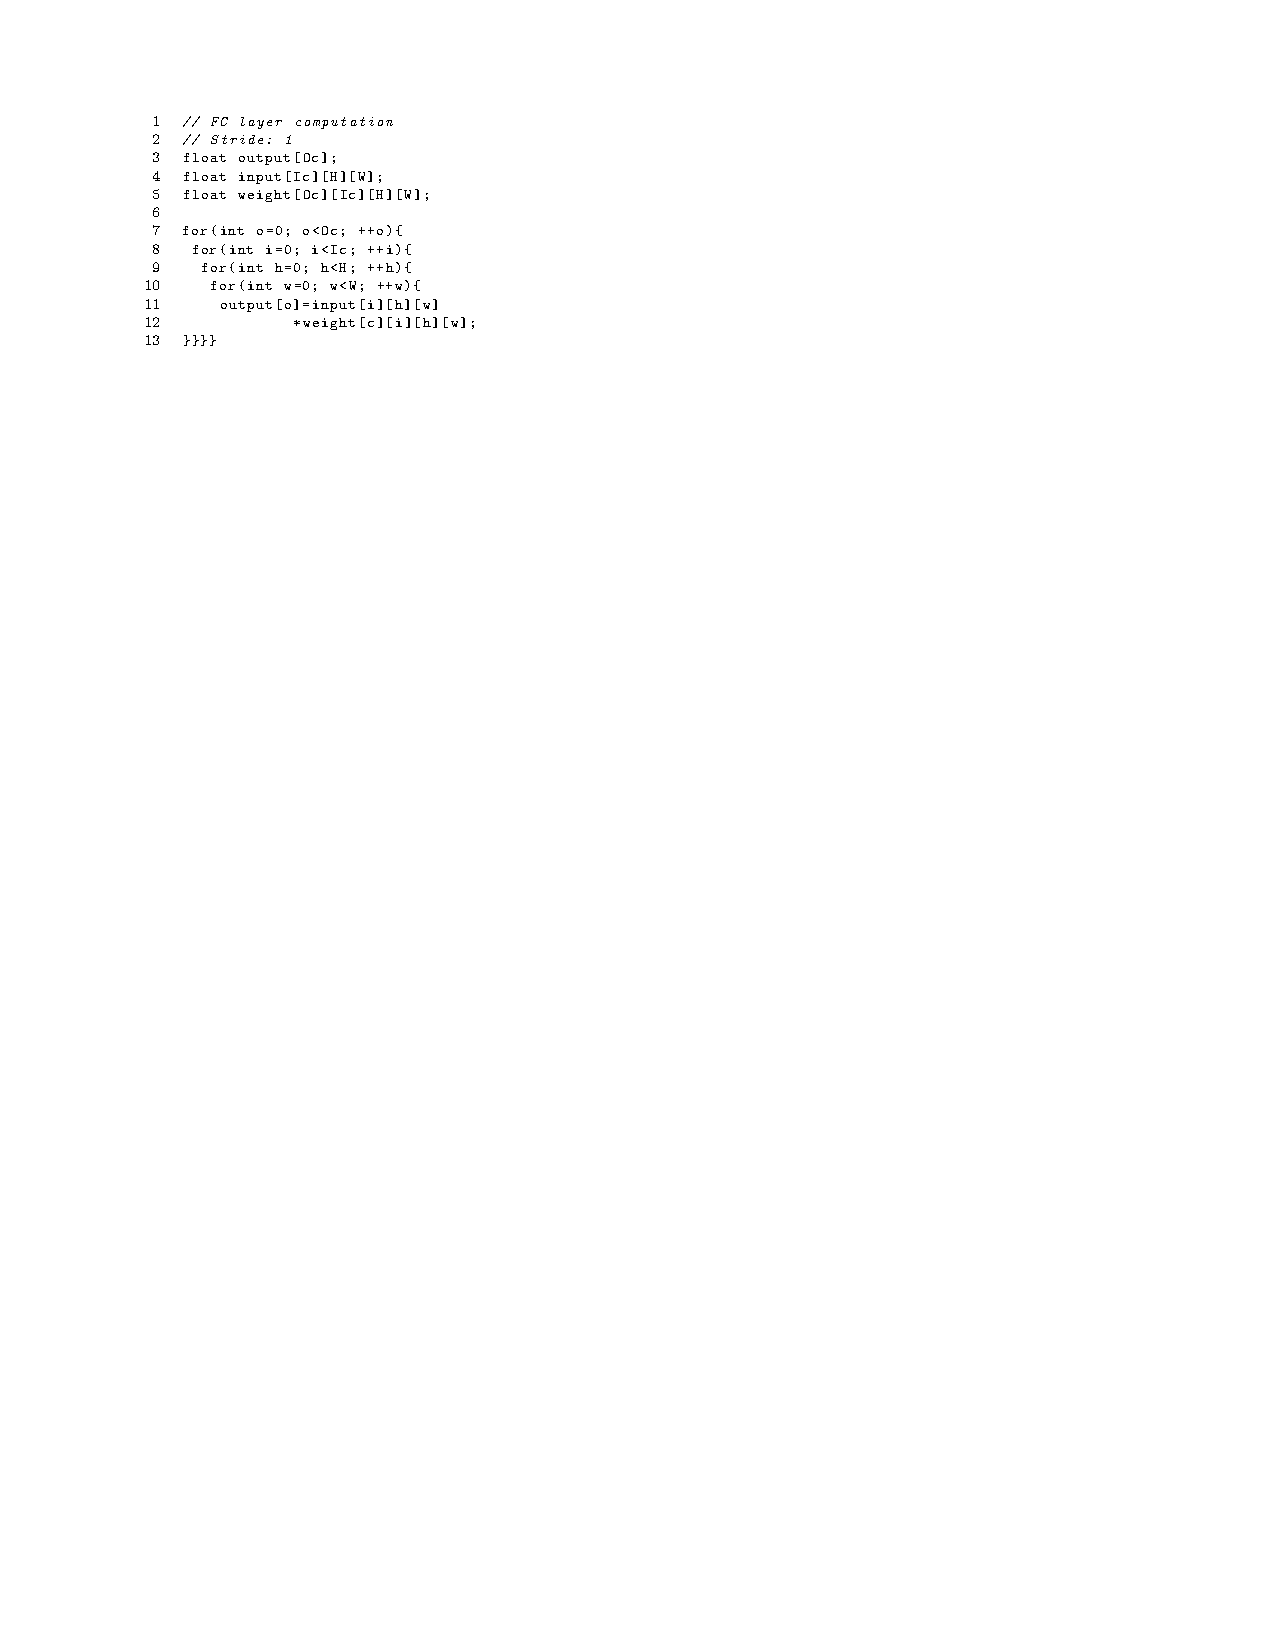
\includegraphics[]{figure/fc.pdf}
        \subcaption{FC layer computation}
    \end{minipage}
    \begin{minipage}[t][]{0.46\linewidth}
        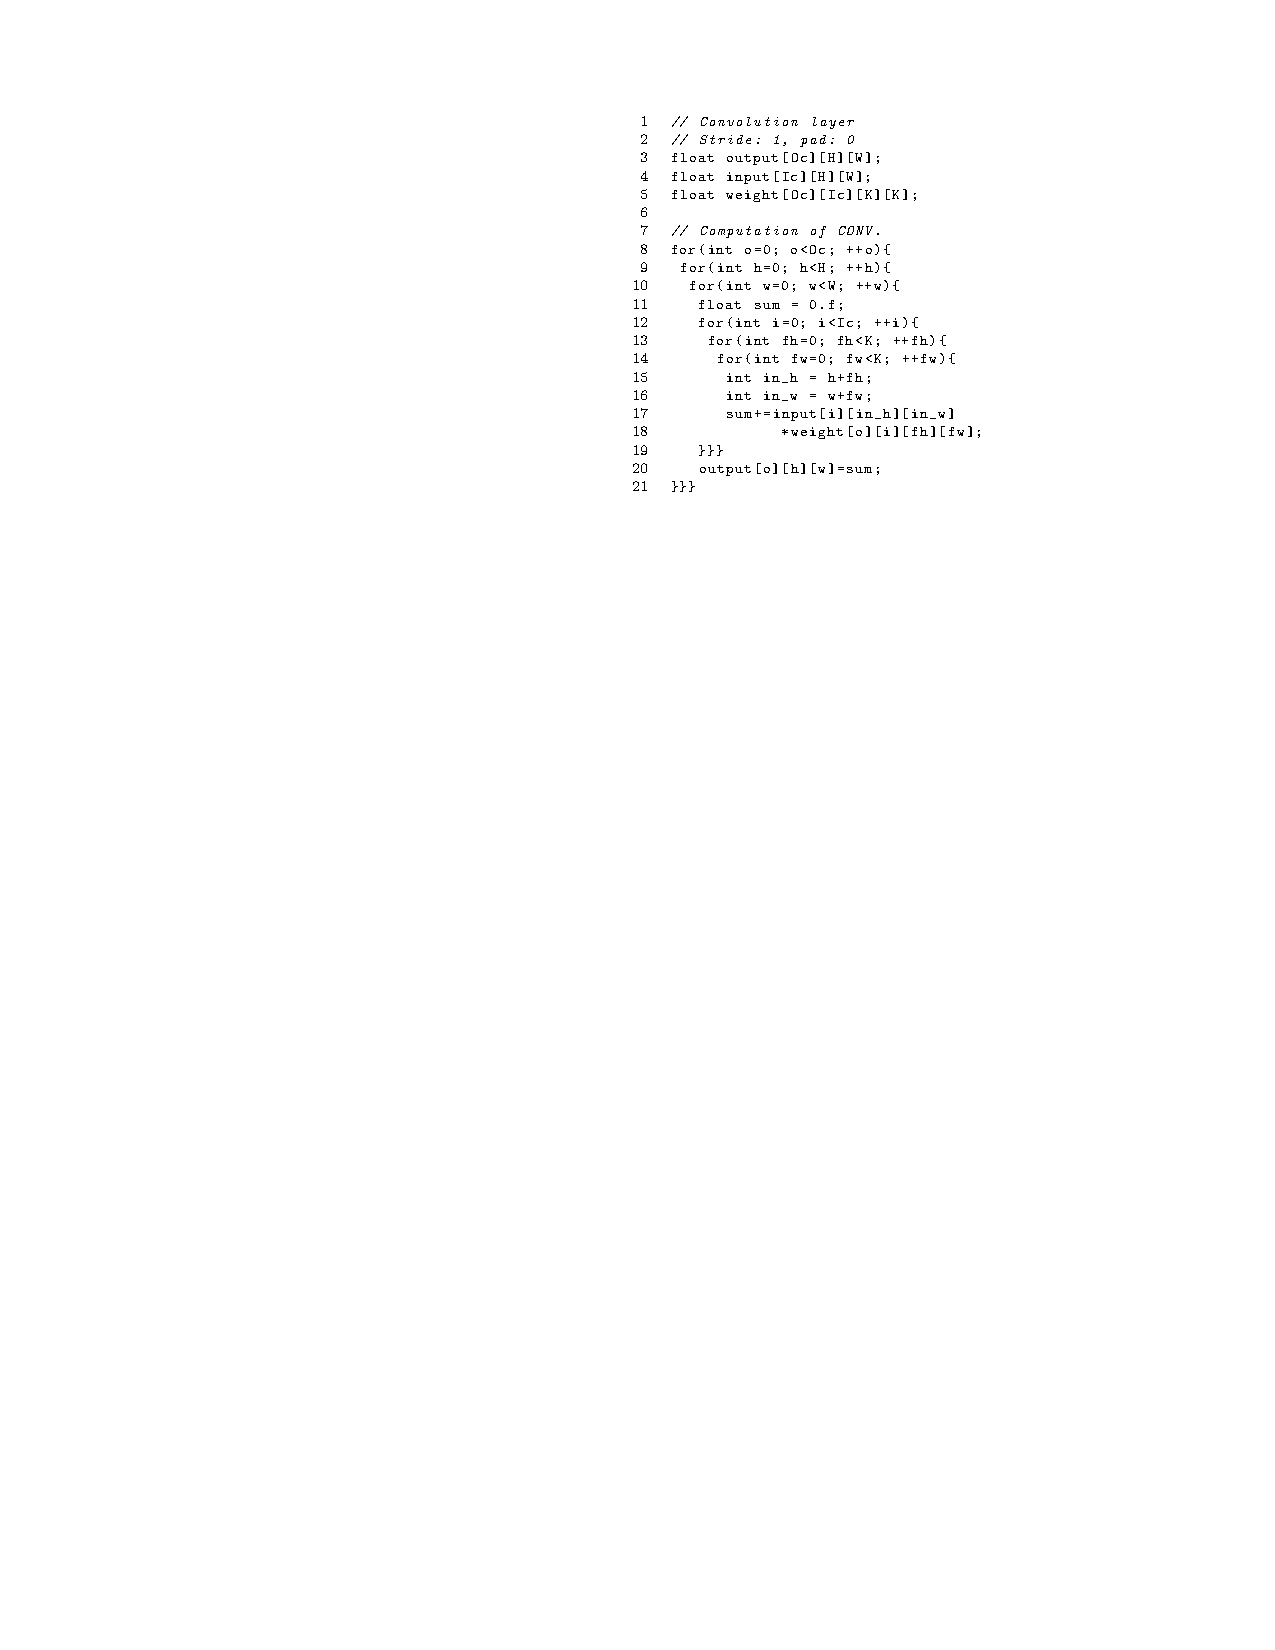
\includegraphics[]{figure/conv.pdf}
        \subcaption{CONV layer computation}
    \end{minipage}
    \caption{FC and CONV layer algorithms}
    \label{fig:ch2:alg}
\end{figure*}

It takes $O_{c}\times O_{h}\times O_{w}$ output multiplying $I_{c}\times I_{h}\times I_{w}$ 
data with $O_{c}\times I_{c}\times K_{h}\times K_{w}$ weight.
The convolution filter slides to each input features and accumulates to make one pixel of output feature.
In this computation, one convolution filter may meet an input pixel twice or more.
As this character, CNNs have two issue that decreases the GPU performance.
% 1. Out-Kernel: Duplication data and # of kernel.
First, there is a lot of duplicated data usage when computing convolution kernel parallel.
Weight is used for all input data and shared as thread index, but input data gets different thread and block index even though the value is same.
Also, GPUs should call lots of kernels computing each convolution as all matrix multiplication is independent.
These kernels are called at GPU core randomly and the memory access pattern is hard to predict what data to gather in the cache.
Besides, the GPU kernel size is bound to the convolution kernel size.
Most CNNs use convolution kernels with the size from $11\times 11$~\mycite{alex2012alexnet} to $1\times 1$~\mycite{he2016resnet} to get accurate features using the data.
This is significantly small compared to the maximum number of thread, usually 512 or 1024, in the kernel on GPU, and it causes the limitation of parallelism executing overall CNNs.
There is another issue when using small convolution kernels.
When it uses general $3\times 3$ convolution kernels, boundary check needs to compute the convolution kernel.
The condition flow in GPU is processed one-by-one execution and it decreases the GPU performance at least twice.
As memory access range is high in CNNs, it shows inefficient memory bandwidth.

\begin{figure*}[t]
    \centering
    \begin{minipage}[t][]{\linewidth}
        \centering
        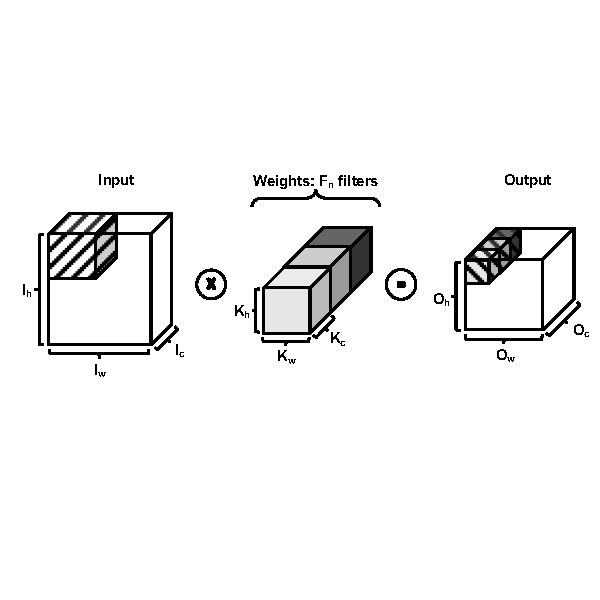
\includegraphics[width=0.9\linewidth]{figure/conv_lower1.pdf}
        \subcaption{Traditional convolution process}
    \end{minipage}
    \begin{minipage}[t][]{\linewidth}
        \centering
        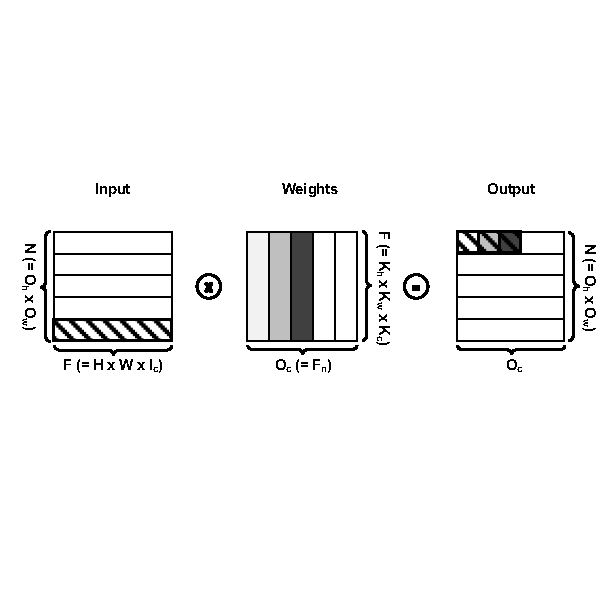
\includegraphics[width=0.9\linewidth]{figure/conv_lower2.pdf}
        \subcaption{Convolution lowering and computation}
    \end{minipage}
    \caption{Convolution structure and computation methodology}
    \label{fig:mot:conv}
\end{figure*}

To optimize memory bandwidth software transformations like convolutional lowering are performed to access memory sequentially.
cuDNN~\mycite{sharan2014cudnn} uses \texttt{im2col} function to convolutional lowering as depicted in Figure~\ref{fig:mot:conv} (b).
\texttt{$I_{c}\times I_{h}\times I_{w}$} input data is changed as \texttt{$I_{c}\times K_{h}\times K_{w}\times I_{h}\times I_{w}$} column.
After transforming, the convolution kernel executes general matrix multiplication (\texttt{GEMM}) with column and weight.
Though convolution lowering requires the amount of memory area due to saving the transformed matrix, it helps to serialize the GPU kernel and increase memory bandwidth as it does not check the boundary of the kernel and fetches continuous data.

\section{DRAM Access Patterns on GPU}
Both CONV (\texttt{im2col + GEMM}) and FC layers demonstrate largely sequential memory access patterns, to maximize DRAM bandwidth and minimize overfetching.
Figure~\ref{fig:ch2:pattern} (a) describes the last FC layer DRAM access patterns.
It reads DRAM on the regular step, which is the same as the stride of each data and weight values.
The output data is written at DRAM, in general, to pass over it to the next layer.
In this example, however, the output number of the last FC layer is only 10 that is small to remain the cache.
Also, it reuses directly at \texttt{softmax} function, which makes probability vector to prediction.
Hence, it does not have to access additional DRAM access to write the output.
In contrast, Figure~\ref{fig:ch2:pattern} (b) is divided into two sides; one for convolution lowering, and the other for matrix multiplication.
There are many DRAM write access (\texttt{0x81520000}~$\sim$~\texttt{0x81820000}) because of saving the transformed matrix data in the memory, while few DRAM read access (\texttt{0x81480000}~$\sim$~\texttt{0x814a0000}) to get original input data.
It might be possible to transform the data layout of a tensor to maximize row buffer locality. 
Although this approach has an advantage for deployment on commodity hardware, 
it is very difficult to implement it as it requires the knowledge of DRAM address mapping. 
Today's GPUs allocate some of the column address bits to high-order bits 
(with optional XOR address hashing) to minimize DRAM bank conflicts. 
This implies that even a simple one-dimensional array is interleaved over multiple banks 
in a non-contiguous manner. Thus, it is very challenging to optimize the data layout purely in software.
Besides, even if the data layout of a single array is carefully optimized, 
there are many concurrent thread blocks accessing the array out of order. 
The state-of-the-art SM scheduler does not take into account DRAM row buffer locality, and its 
non-deterministic behaviors make DRAM locality optimization in software even more difficult.

\begin{figure}[t]
	\centering
	\begin{minipage}{\textwidth}
	    \centering
    	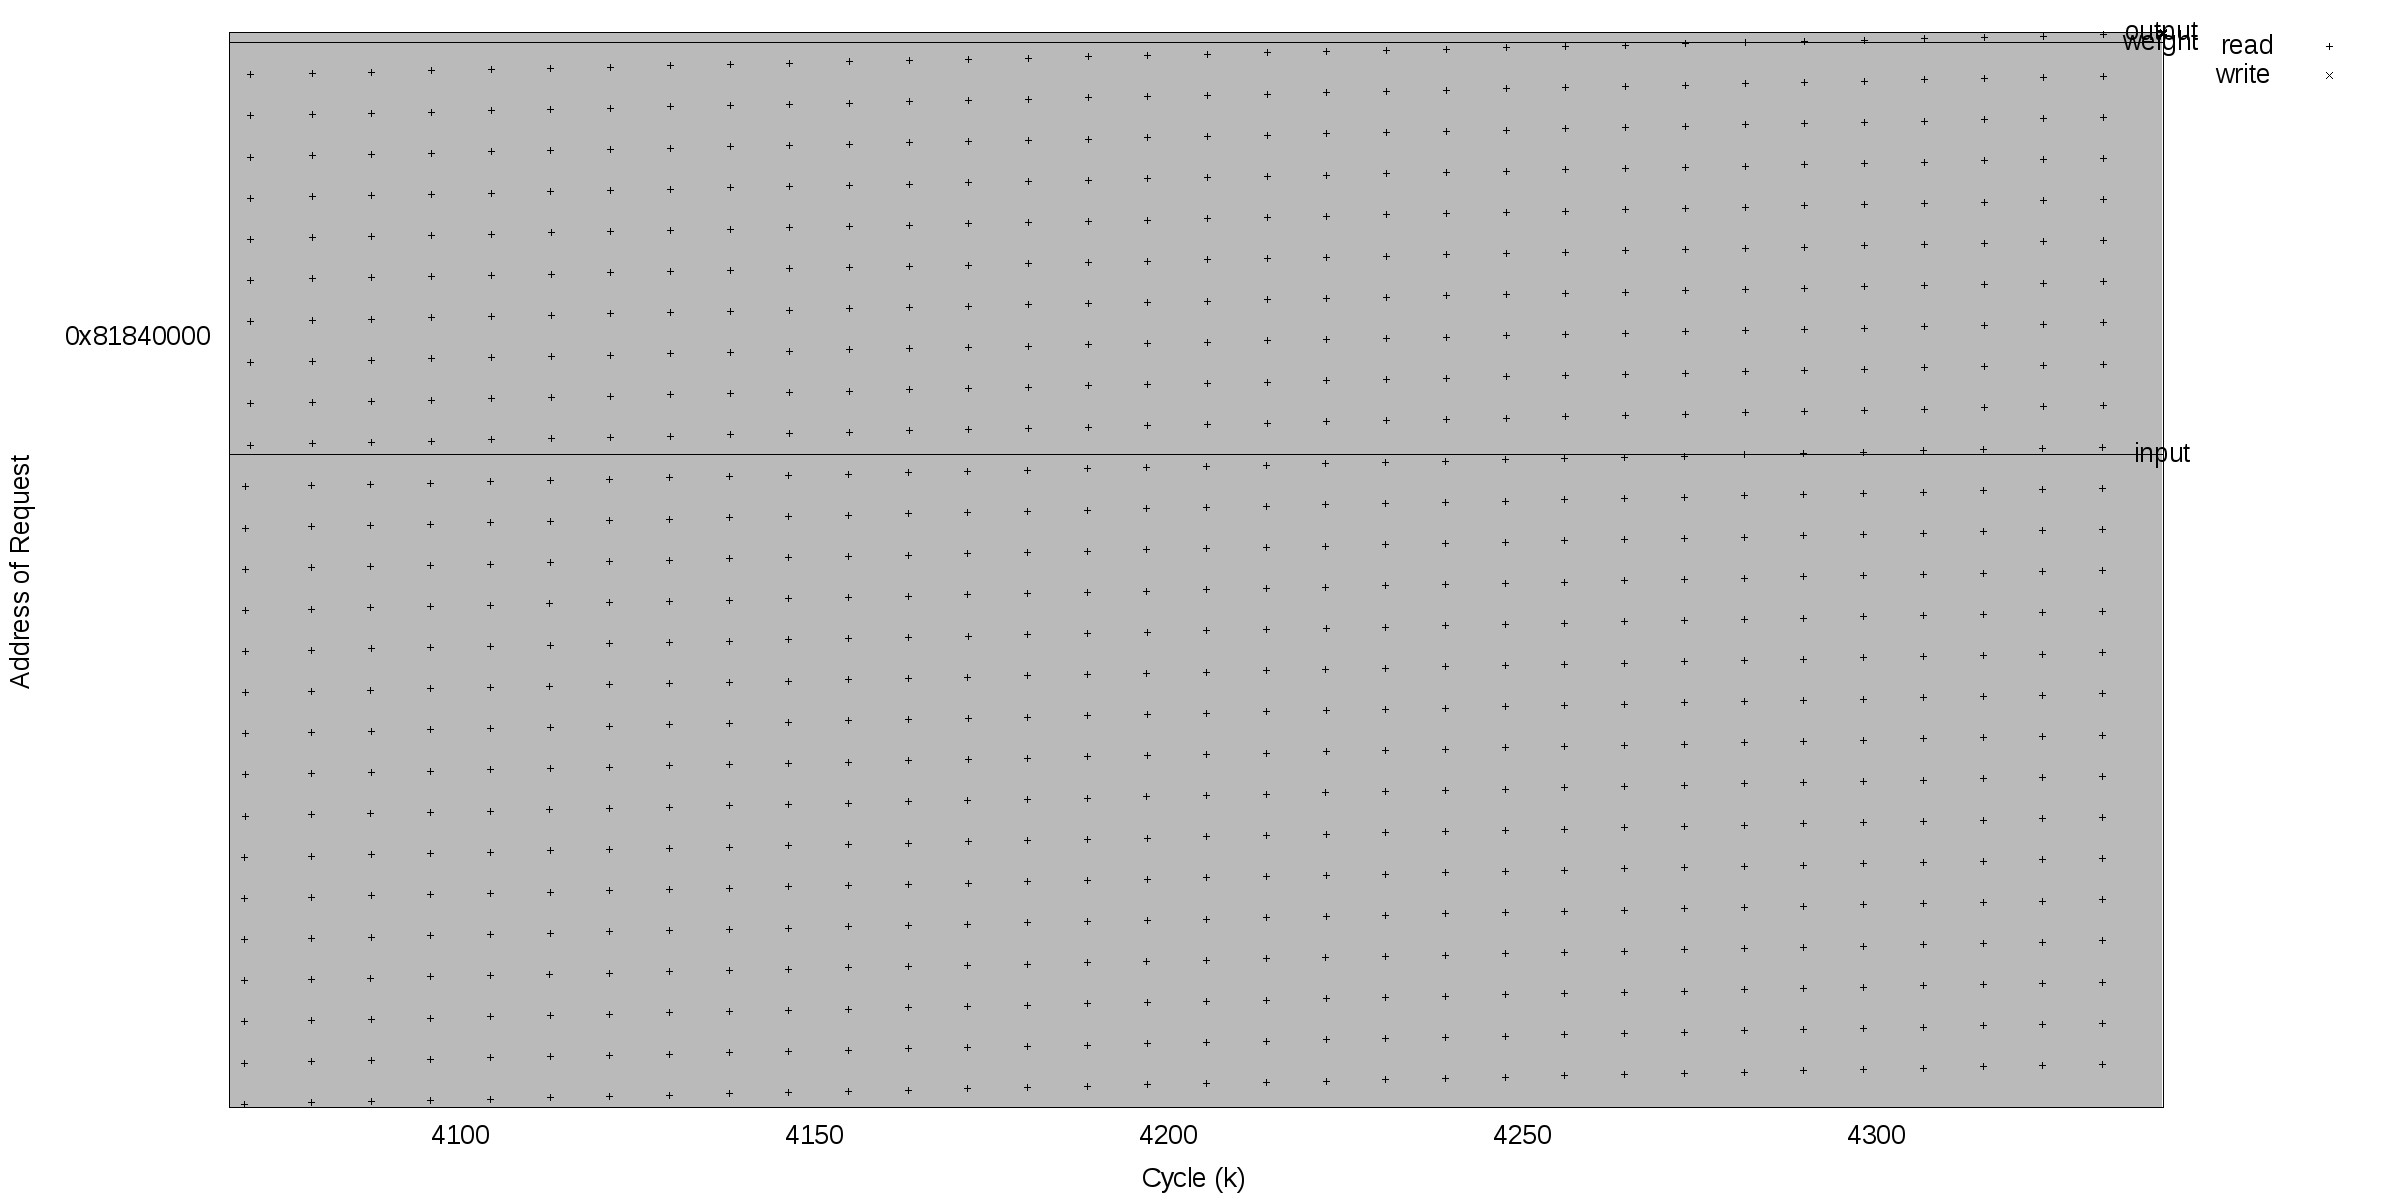
\includegraphics[width=0.80\textwidth]{figure/fcpat.png} 
    	\subcaption{FC layer}
    \end{minipage}	
	\begin{minipage}{\textwidth}
	    \centering
    	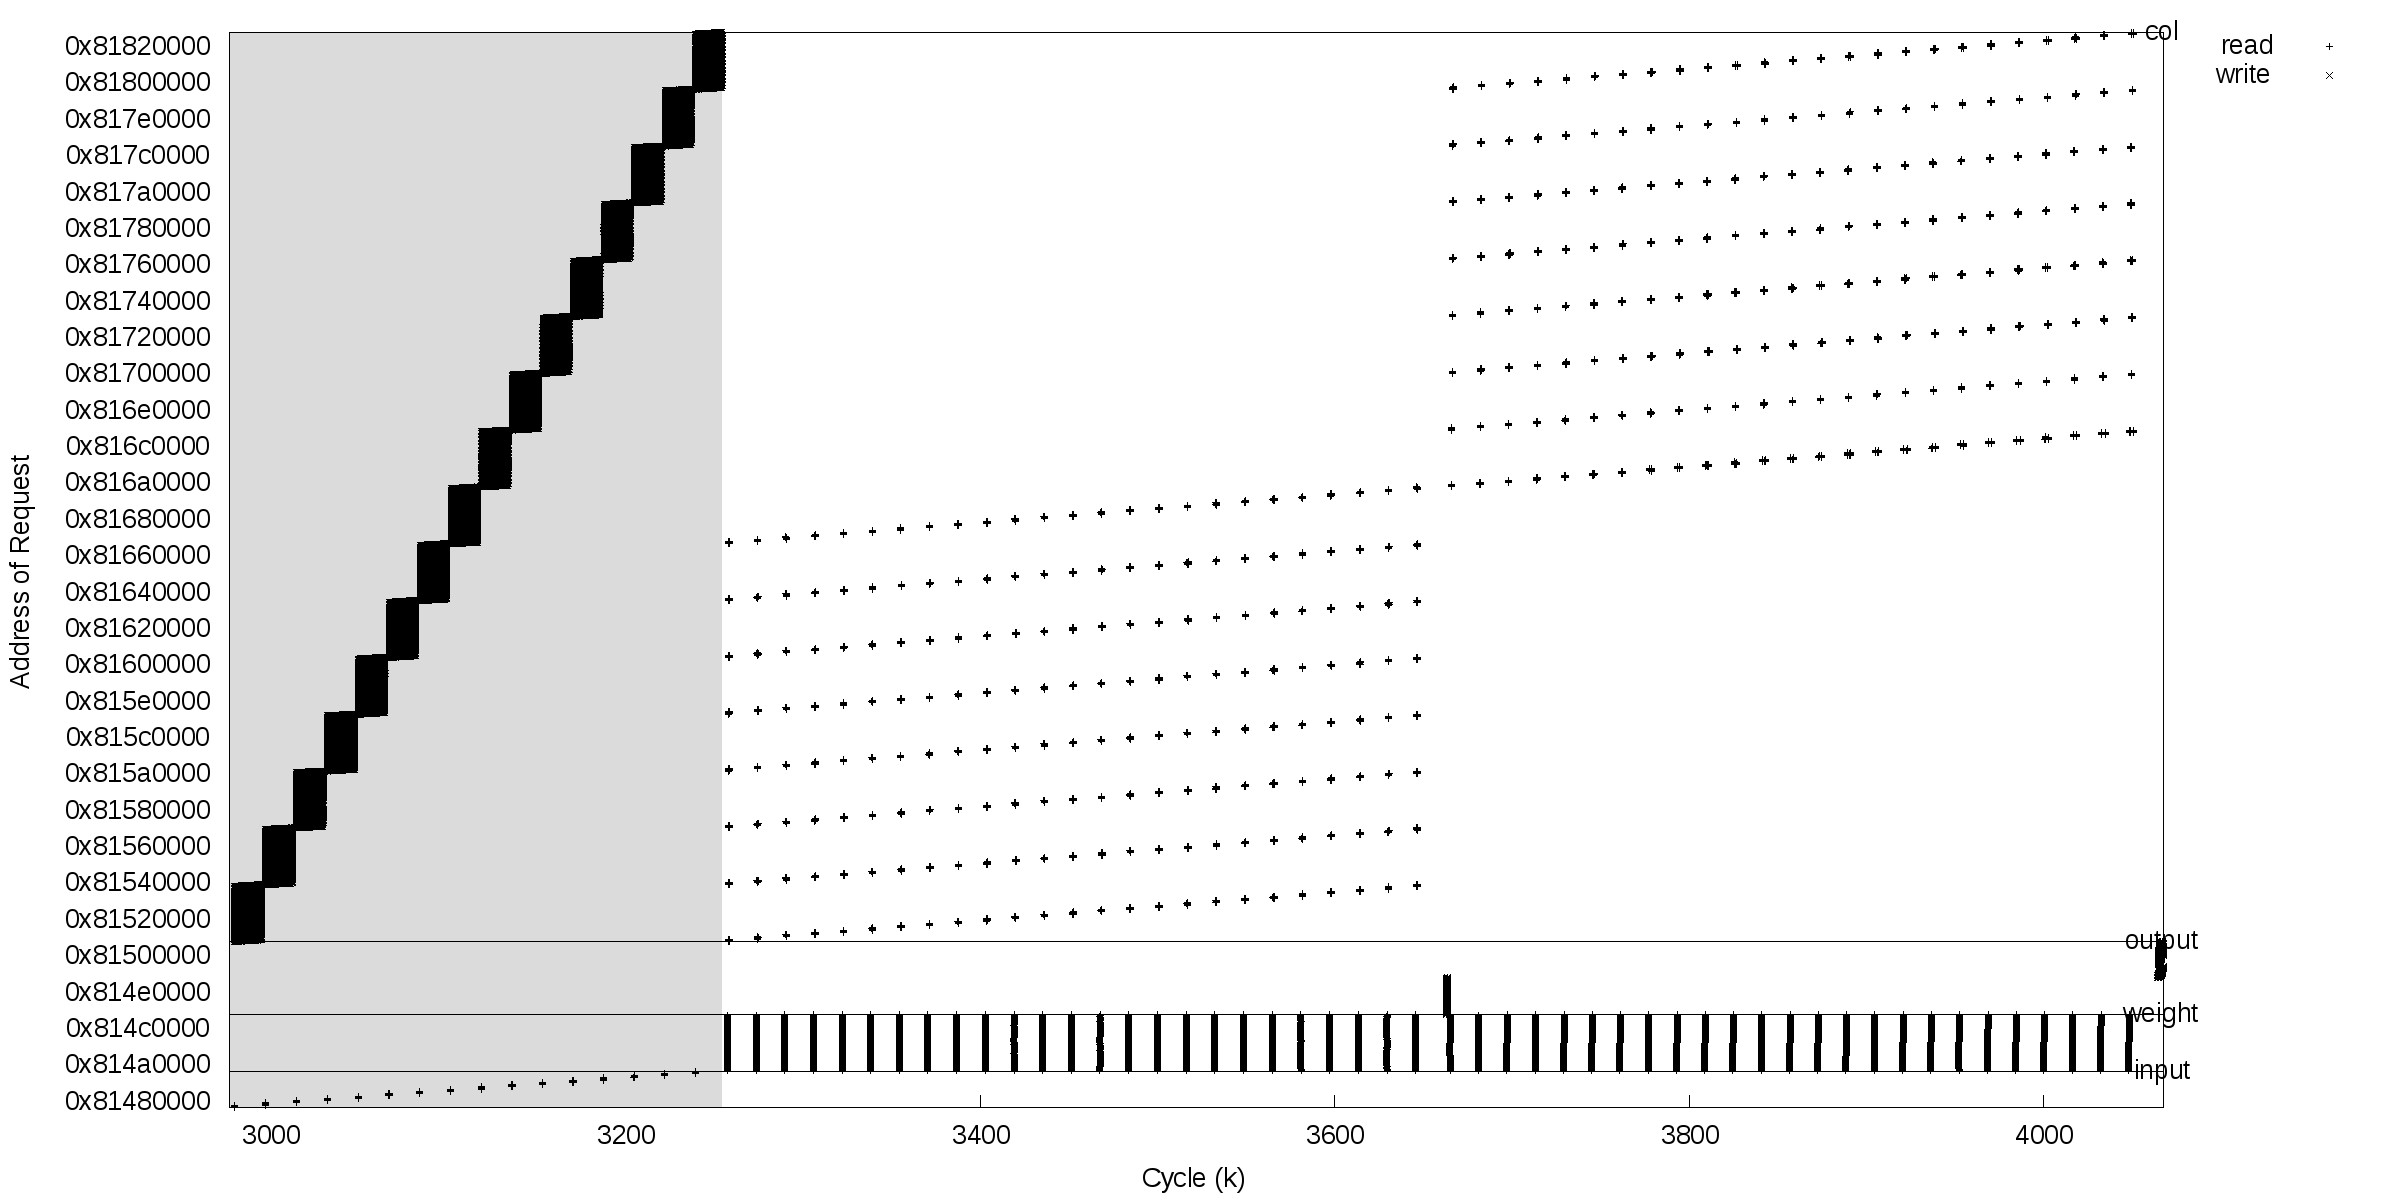
\includegraphics[width=0.80\textwidth]{figure/convpat.png}
    	\subcaption{CONV layer}
    \end{minipage}
	\caption{DRAM access patterns executing cuda-convnet on each layer}
	\label{fig:ch2:pattern}
\end{figure}

\section{Partial Row Activation}
Partial row activation scheme is a well-known technique to mitigate the overfetching problem.
Earlier works including Fujitsu Fast Cycle RAM (FCRAM)~\mycite{fcram}, fine-grained activation 
DRAM~\mycite{copper2010fineact} and~\mycite{udipi2010rethinking}.
These works can attain plenty of activation energy saving. 
However, that comes with a significant area overhead due to many peripherals 
(i.e., lower cell efficiency) which support fine-grained activation.
Fine-grained activation~\mycite{copper2010fineact} added a one-hot decoder and a single AND gate to the
wordline of each division in a row. The division of row is selected and activated when earning both 
row and column address. Using Posted-CAS command, DRAM controller sends row and column command 
back-to-back cycle. It reduced the DRAM power by up to 40\%. 

Selective bitline activation (SBA) and single subarray access (SSA)~\mycite{udipi2010rethinking}
fundamentally re-organized the layout of DRAM arrays and the mapping of data to these arrays so that an
entire cache line was fetched from a single subarray. Introducing new protocol existing JEDEC DRAM
interface called Posted-RAS, which hold the row address until the column address arrives to activate
the bitline selectively. It reduced dynamic and background energy about $5\times$.

More recent work addresses these problems but requires changes to the DRAM interface and protocols.
\mycite{yb17, Zhang14, halfpage, SALP12, subchannel17, connor2017finedram}
Many of these proposals make use of memory controller side information
when issue column commands (posted-CAS \mycite{postedcas}) or introduce new DRAM commands. 
\mycite{yb17}, for example, partial row activation mask is required
from the memory controller after row command issued to activate the dirty cache block.

Half-DRAM~\mycite{Zhang14} proposed a reconstructed DRAM architecture to address the row overfetching
problem. 
By splitting one mat into two parts, it enables half row activation which is almost no bandwidth
loss while achieving row activation power saving. As to the extending Half-DRAM which can perform
one-eighth row activation, it has a relatively large area overhead.

Fine-grained DRAM and subchannel~\mycite{connor2017finedram, subchannel17} proposed a new high-bandwidth
DRAM architecture to improves bandwidth by four times and energy efficiency by twice compared to existing
HBM2 reorganizing HBM2 channel structure into the narrow parallel channel to mitigate latency overhead 
due to the narrow path of the fine-grained activation structure. 
But these works require significant modification of microarchitecture of DRAM core that incurs 
the area overhead up to 10\%.

\section{Performance/Area Trade-off in Partial Activation}
 Many previous studies identify the row access energy as a major component of DRAM dynamic energy~\mycite{udipi2010rethinking, halfpage}. As a result, there are multiple proposals on partial row activation of DRAM. However, as we hinted earlier, most of these works require a substantial area overhead or changes to the DRAM protocol. This is because of a trade-off between cost (area) and performance. In a conventional DRAM architecture, a DRAM row is striped across multiple DRAM cell arrays, or \emph{mats}. Upon an {\tt ACTIVATE} command a whole row of each mat is latched. Then, when a {\tt READ} command arrives, each mat provides the same number of bits (i.e., 16 bits in HBM2 pseudo-channel mode) based on the provided column address from latches and outputs them to the bus. One potential way to enable partial activation is to segment every single row of each mat and activate only part of the selected row within a mat. However, this requires adding a large number of AND gates and local wordlines to incur huge area overhead~\mycite{udipi2010rethinking}. Another potential way is to re-arrange DRAM column data layout so that a single mat (or a few mats) contains the whole contents of a column in a row. This design can implement partial activation by letting only a single mat to be activated but it incurs a performance overhead as such design needs to output data through a narrow path between a single mat and the I/O, thus incurring serialization delay. An alternative to the previous approach is to increase the width of a path between a single mat and the bus to avoid performance penalty, which also results in a large area overhead.

\section{Latency-Tolerance of Deep Learning Workloads on GPU}
\begin{figure}[t]
	\centering
	    \centering
    	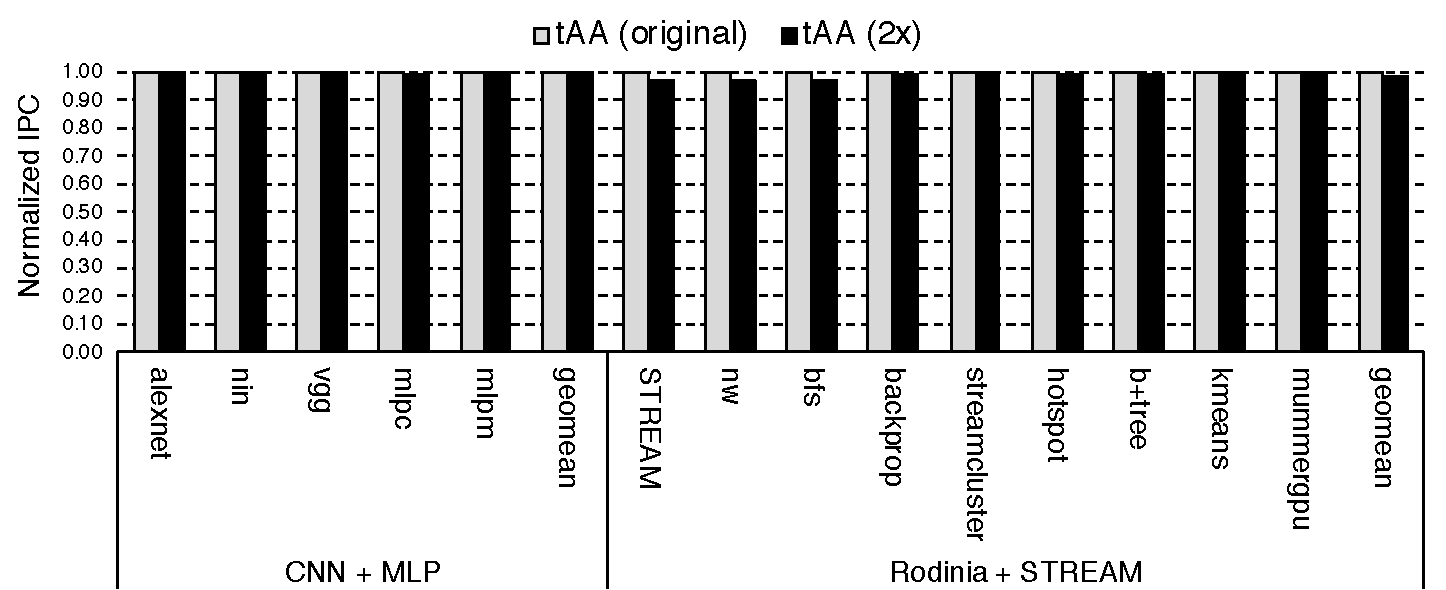
\includegraphics[width=0.90\textwidth]{figure/taa_long.pdf} 
	\caption{Performance degradation with longer column latency ({\tt tAA})}
	\label{fig:ch2:perfhit}
\end{figure}

 One important characteristic of the emerging GPU workloads is that they are tolerant to a long memory latency. Such workloads are often embarrassingly parallel and GPU exploits this characteristic by scheduling multiple warps (e.g., 64) to a single streaming multiprocessor (SM). When a warp in the SM cannot execute due to memory latency, another warp in the SM will be run instead. With this mechanism, the SM can effectively utilize its compute units and operate at a near-perfect efficiency despite the presence of long-latency memory operations. Figure~\ref{fig:ch2:perfhit} demonstrates the latency tolerance of two popular types of deep learning workloads, convolutional neural networks (CNNs) and multi-layer perceptrons (MLPs), by presenting the performance impact of increasing the {\tt tAA} timing parameter (i.e., internal read command to data output) by $2\times$. As shown in the figure, all five workloads show no performance degradation. The other conventional GPU workloads also show at most 4\% performance degradation. Note that this does not mean that the memory system is not important for GPU workloads. While they are less sensitive to memory latency, most GPU workloads, due to its high degree of parallelism, require large memory bandwidth. Based on this observation, we propose to trade DRAM latency for energy savings in this work.



%We need a more practical partial row activation scheme which has low area/power overhead without
%requiring changes to the existing DRAM interface.
%Unlike these previous works, our work avoids area overhead and significant interface change 
%while achieving substantial energy saving by exploiting the fact that most GPU workloads are not
%sensitive to memory latency.



\chapter{Practical Partial Row Activation}
\section{Overview}

The baseline HBM2 device is organized as follows: 
base and core die slice which is stacked up to 8-Hi slices. 
The core die slice has 4 channels interconnected by TSV as shown Figure~\ref{fig:ch3:basearch}, 
Each of which has four quadrants with 16 banks/quadrant. 
Each quadrant, a channel is assigned 128 TSV I/Os in the TSV area across the core slice. 
Currently, we assume that our baseline HBM2 device consists of 4-Hi slices. 
So individual channel has 32 banks divided into upper and lower slice group.

We introduce two terminologies to the baseline HBM2 design: \textit{sectors} and activation bit vector. 
The \textit{sector} is a minimum activation granularity of row buffer. 
We divide row buffer into 8~\textit{sectors} from previous partial activation schemes from \mycite{yb17} and \mycite{Zhang14}.

\begin{figure}[th]
    \centering
        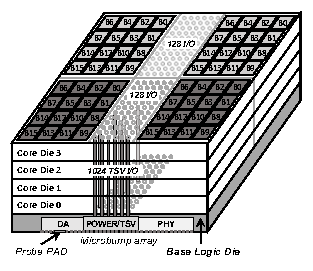
\includegraphics[page=1,width=0.5\linewidth]{figure/baseline_HBM2.pdf}
    \caption[Baseline HBM2 architecture]{Baseline HBM2 architecture\footnotemark{}}
    \label{fig:ch3:basearch}
\end{figure}

\section{Bank Structure}

\begin{figure}[th]
    \centering
        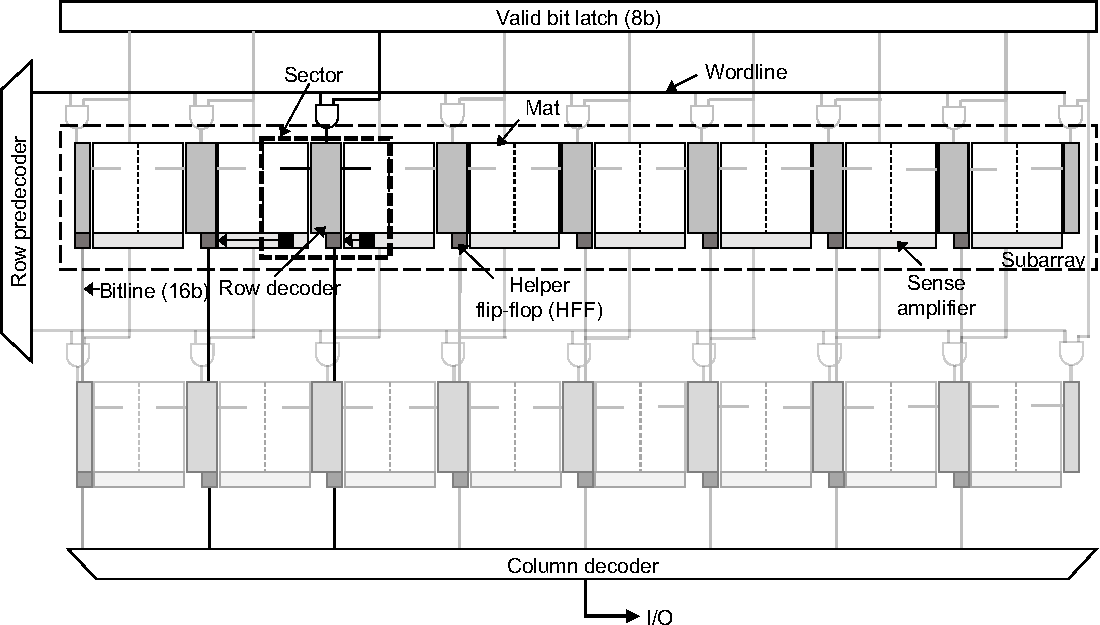
\includegraphics[width=\linewidth]{figure/bank_structure_vfin.pdf}
    \caption{Detailed view of PPA bank architecture}
    \label{fig:ch3:bankstruct}
\end{figure}

\footnotetext{Reproduced from \mycite{IMW17}} % HBM2 PKG fig citation
Figure~\ref{fig:ch3:bankstruct} 
shows the structure of a bank for our proposed DRAM architecture based on HBM2. A single bank consists of multiple subarrays, each of which is further divided into 8 mats sharing the same global word line. With the row size of 1KB, activating a single mat reads out 128B of row data, which is a common cacheline size for GPUs. Exploiting this characteristic, we re-organize the column address mapping of mats so that one mat houses a whole 32B column. To enable an activation of a single mat (instead of all eight), we simply add AND gates to the global word line. Such design increases the time to process a {\tt READ/WRITE} command by 14 memory cycles as it takes 14 extra cycles to burst out a 32B atom through a 16-bit-wide datapath (16 memory cycles in total) instead of a 128-bit-wide datapath (2 memory cycles in total).

To mitigate the effect on {\tt READ/WRITE} processing time from a narrower path to I/O, we also employ a proposal similar to half-DRAM~\mycite{Zhang14}. The main intuition of the Half-DRAM proposal is that it is possible to utilize two set of bitlines (and helper flip-flops (HFFs)) for activating a single DRAM cell worth of data by making a row decoder drives two half mats (the right half of the mat on the left and the left half of the mat on the right) instead of a single mat. As shown in Figure \ref{fig:ch3:bankstruct}, two half mats now utilize two sets of the 16 bitlines and this reduces the {\tt READ/WRITE} processing time to 8 memory cycles (i.e., 6-cycle increase). Note that we modify column mapping of mats so that a whole column address fits in two corresponding half mats. Throughout the paper, we call these two corresponding half mats a {\it sector} as shown in Figure~\ref{fig:ch3:bankstruct}.

To handle this increase in {\tt READ/WRITE} command processing time, we need to adjust DRAM's timing parameters. First, timing parameter {\tt tAA}, which represents the time between the read command and the first data output on bus, needs to be increased as the proposed bank structure requires extra cycles to output the data.  So {\tt tAA} is increased by 6 memory cycles. 
\begin{figure}[t]
    \centering
        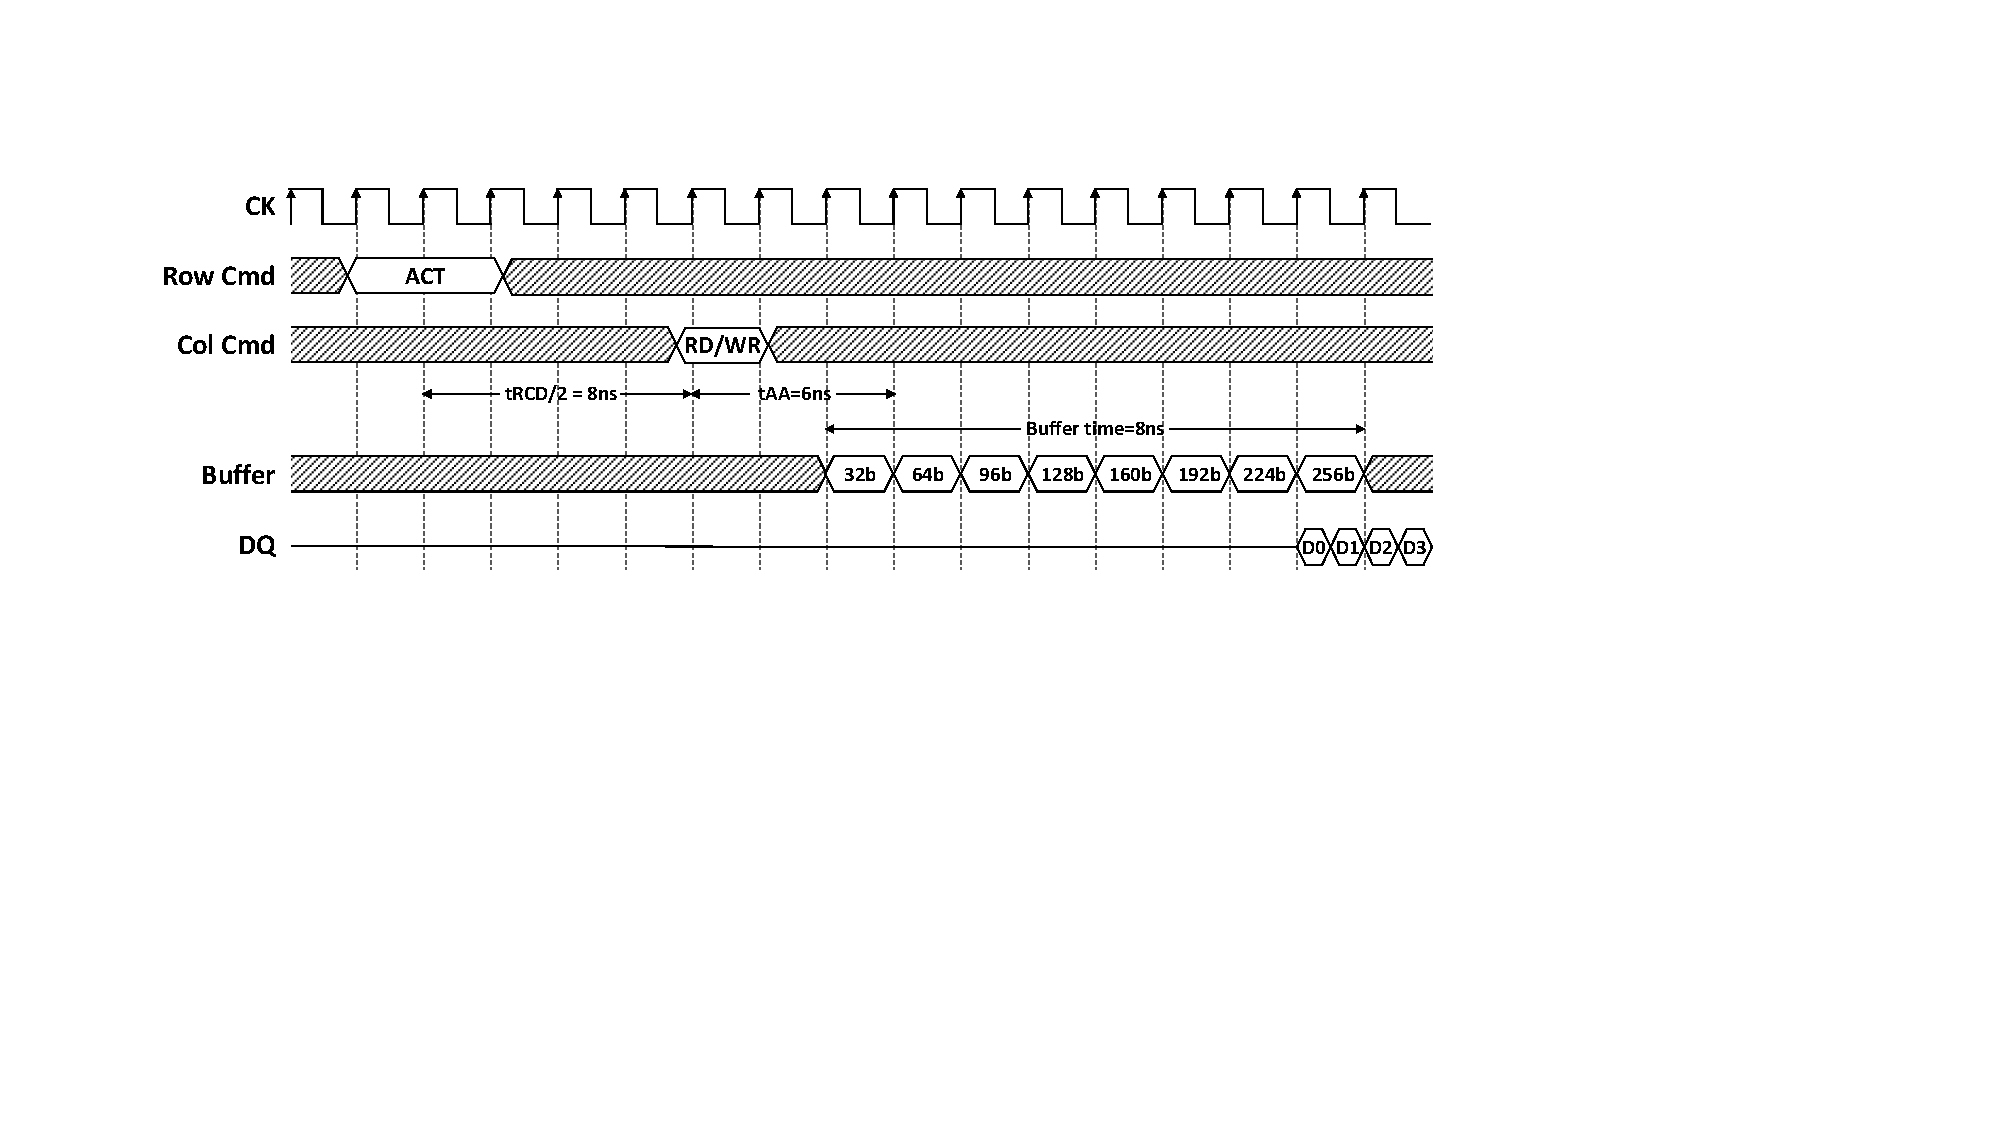
\includegraphics[width=\linewidth]{figure/data_fetch_time.pdf}
    \caption{Data fetch timing diagram through the narrow bitline}
    \label{fig:ch3:datfetch}
\end{figure}

Figure~\ref{fig:ch3:datfetch} above describes how the {\tt tAA} timing is lengthened 
when data being fetched by a cycle-by-cycle waveform. After corresponding {\it sector} activated, 
the 16-bit-wide bitlines on both sides are utilized to buffer the requested 32B data. 
The data is fetched 32 bits per cycle, and it takes 8 cycles to fetch 256 bits.
Since the first cycle of fetch data and {\tt tAA} timing can overlap, and the last fetch and two bursts 
can overlap, thus it takes a total of 6 cycles to buffer the data through the narrow bitline.

The timing between column commands to the same bank has to be increased. While a memory controller compliant to HBM standards already has {\tt tCCD}, column command to column command delay, we need a variation of this because we only need to increase the delay between column command to column command {\it to the same bank}. We denote this parameter {\tt tCCD}$_S$ and set it to {\tt tCCD}+6. This requires a slight timing change to the memory controller. Lastly, other {\tt READ/WRITE} related delays (e.g., {\tt tWR}, {\tt tWTR}, and {\tt tRTP}) needs to be increased by six cycles as well.

While these mechanisms reduce the peak bank bandwidth by up to 4$\times$ since the time it takes to handle a single {\tt READ/WRITE} command increases to 8 cycles from 2 cycles. However, this often does not lead to a decrease in overall memory bandwidth since HBM2 specification over-provisions DRAM banks. For example, the evaluated configuration includes 32 banks per channel, where each bank can provide up to 128 bits/cycle. On the other hand, each channel, despite having 32 banks, supply data at 256 bits/cycle. Assuming balanced distributions across 32 banks, each bank only needs to supply 8 bits/cycle to saturate the channel bandwidth. In other words, each bank achieving 1/16$\times$ of its peak throughput is enough to saturate the channel in this case. For this reason, although our proposed bank structure reduces the peak throughput of a single bank by 4$\times$, it is unlikely to affect the overall memory throughput, which is often first limited by channel throughput.

\begin{figure}[b]
    \centering
        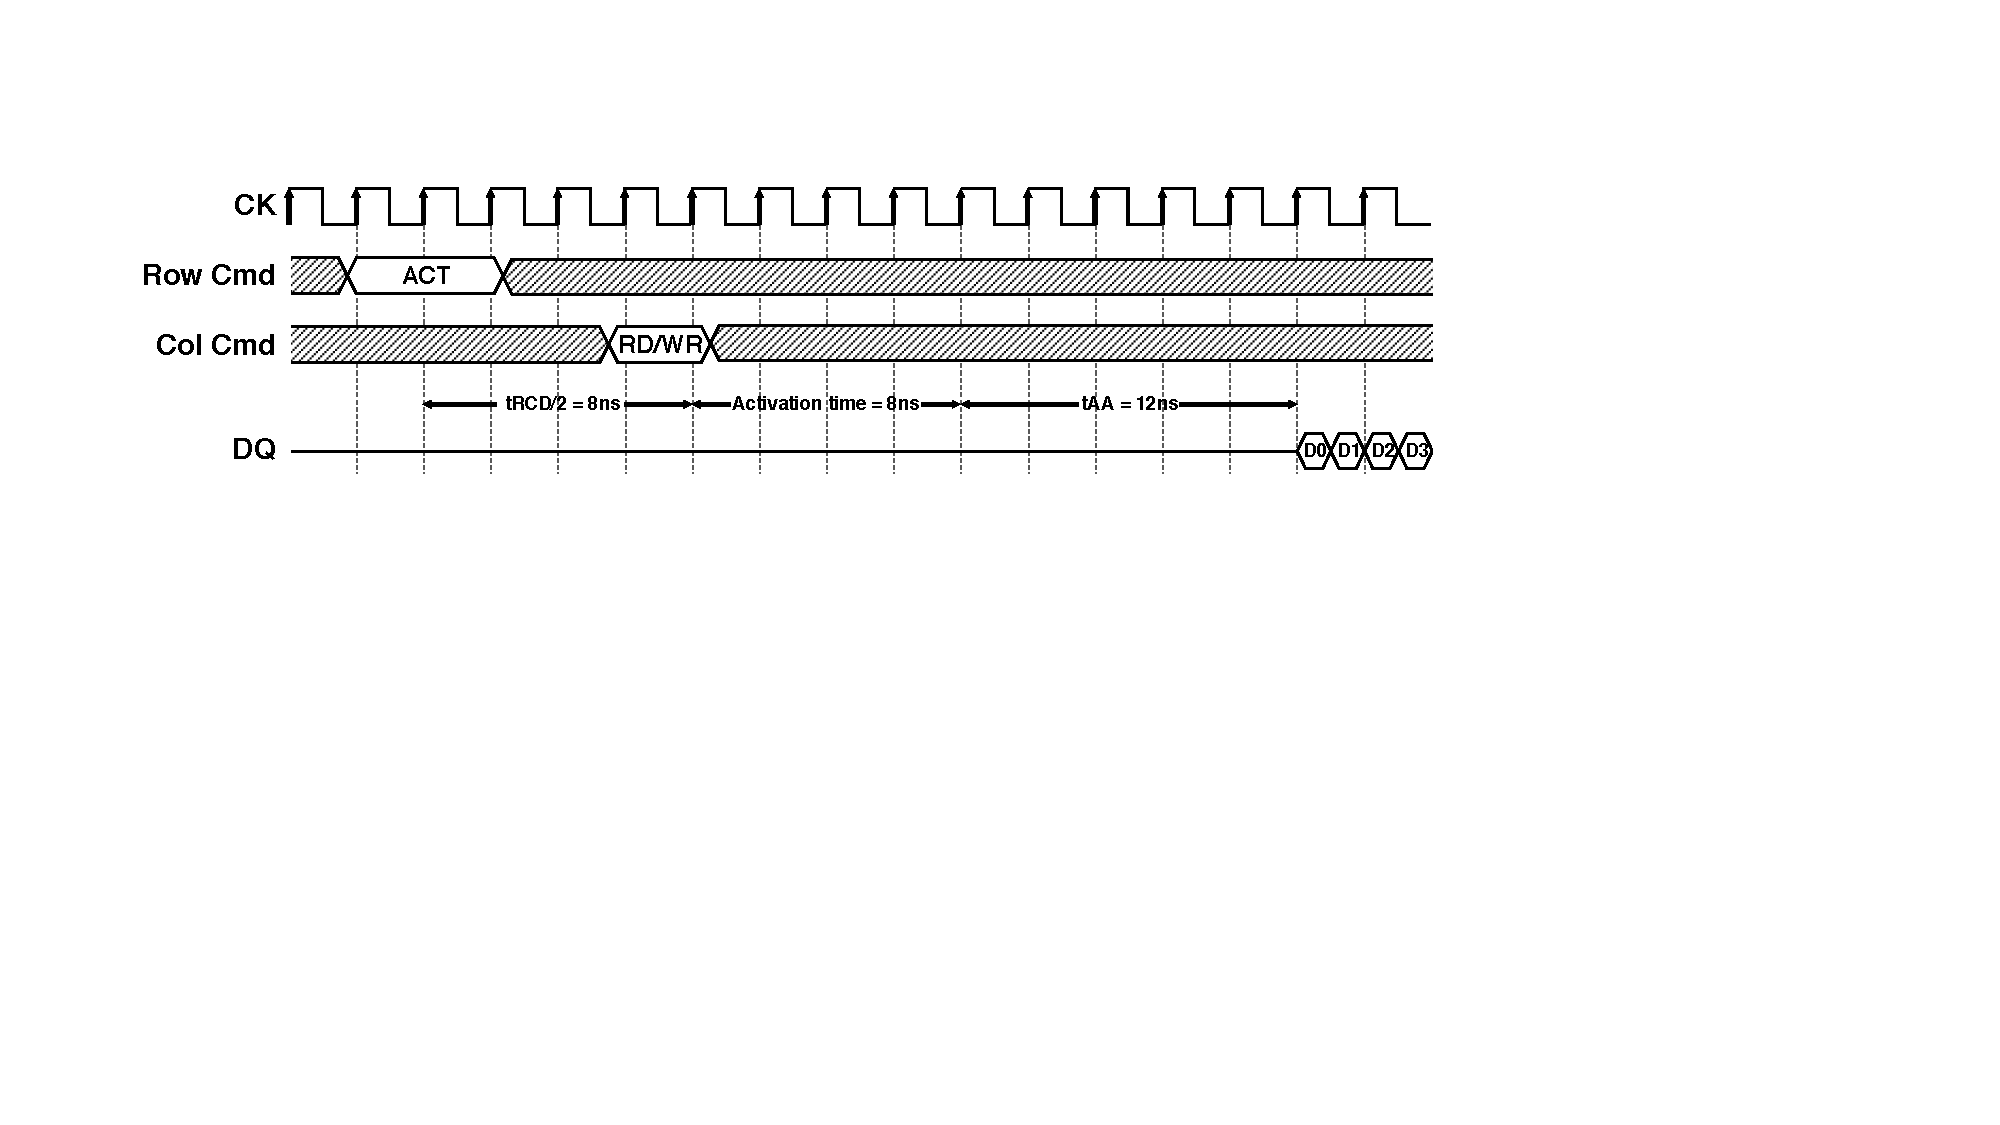
\includegraphics[width=\linewidth]{figure/waveform_del_act.pdf}
    \caption{Waveform of proposed delayed activation}
    \label{fig:ch3:delact}
\end{figure}

\section{Delayed Activation}
To specify which {\it sector} to activate we use delayed activation. When a DRAM device receives {\tt ACTIVATE} commands, the DRAM device decodes row address as usual but does not actually perform an activation and buffer the row address. Instead, the activation happens when a column command arrives. Once a column command (i.e., {\tt READ/WRITE}) arrives, the column address is first decoded and it is used to determine which DRAM {\it sector} it should activate. Then, a partial activation for that particular {\it sector} is performed and followed by actual READ/WRITE operation. Figure \ref{fig:ch3:delact} shows how this delayed activation scheme affects DRAM timing. First, since {\tt ACTIVATE} does not actually perform an activation, {\tt tRCD} becomes shorter (by half according to our estimation using CACTI-3DD \mycite{cacti3dd}). At the same time, since the activation happens in column commands, {\tt tAA} (i.e., the timing of read command to the first output data on the bus) and {\tt tWL} (i.e., the timing of write command to the first input data on the bus) should be increased by the reduced {\tt tRCD} amount. In our configuration, {\tt tRCD} is originally set to 16ns and thus {\tt tRCD} is reduced by 8ns while {\tt tAA} and {\tt tWL} are increased by 8ns. This scheme basically avoids unnecessary activation at the expense of potential 8ns extra latency for {\tt READ} and {\tt WRITE} command. The rationale behind this scheme is that such a minor increase in DRAM latency does not usually affect the performance of the latency-tolerant GPU workloads.

%The main idea of delayed activation is that we can only activate the exact amount of data we need in an on-demand basis. 
%According to the FR-FCFS policy, column accesses to the open row are prioritized over those to other rows.
%When a DRAM receives ACTIVATE commands, the DRAM device decodes row address as usual but does not actually perform an activation and buffer the row address. 
%Instead, the activation happens when a column command arrives. 
%Once a column command (i.e., {\tt READ/WRITE}) arrives, the column address is first decoded, and it is used to determine which DRAM \textit{sector} it should activate. 
%Then, a partial activation for that particular \textit{sector} is performed and followed by actual {\tt READ/WRITE} operation.
%When a DRAM request is headed to another row, a precharge must be performed first 
%as if a normal row buffer conflict occurred.
%
%Figure~\ref{fig:ch3:delact} shows how this delayed activation scheme affects DRAM timing. 
%First, since ACTIVATE does not actually perform an activation, $t_{RCD}$ becomes shorter 
%(half according to our estimation using CACTI-3DD~\mycite{cacti3dd}). At the same time, since the
%activation happens in column commands, $t_{AA}$ (i.e., the timing of read command to the first output 
%data on the bus) and $t_{WL}$ (i.e., the timing of write command to the first input data on the bus)
%should be increased by the reduced $t_{RCD}$ amount. 
%In our configuration, $t_{RCD}$ is originally set to 16ns and thus $t_{RCD}$ is reduced by 8ns while $t_{AA}$ and $t_{WL}$ are increased by 8ns. 
%This scheme basically trades-off an ability to avoid unnecessary activation at the expense of potential
%8ns extra latency for {\tt READ} and {\tt WRITE} command. 
%The rationale behind this scheme is that such a minor increase in DRAM latency does not usually affect the performance of latency-tolerant GPU workloads.


\chapter{Evaluation}
\begin{table}[t]
\centering
\footnotesize
\begin{tabular}{|l|l|}
\hline
  \textbf{Platform} & \textbf{Nvidia GTX 780TI} \footnotemark{} \\ \hline
  \begin{tabular}[c]{@{}l@{}}Warp size\\ \# of SM cores\\ Execution model\\
                              Max warps per SM\\ Size of register file\\ \# of register banks\\
                              Warp scheduler\end{tabular}
                              & \begin{tabular}[c]{@{}l@{}}32\\ 16\\ In-order\\
                              64\\ 256KB (per SM)\\ 24\\
                              Greedy then oldest\end{tabular} \\ \hline
  \begin{tabular}[c]{@{}l@{}}Shared memory\\ L1 Cache\end{tabular}
                              & \begin{tabular}[c]{@{}l@{}}48KB\\ 16KB\end{tabular} \\ \hline
  L2 Cache & 1536KB \\ \hline
\end{tabular}
\caption{Platform parameters}
\label{tab:metho:platform}
\end{table}
\footnotetext{GPU architecture parameter from \mycite{APCM}}

\section{Methodology}
We evaluate the proposed scheme using GPGPU-Sim~\mycite{bakhoda2009analyzing}. 
Table~\ref{tab:metho:DRAMparam} shows the configuration we used for the simulation. We assume HBM2 device architecture based on a recent HBM2 design~\mycite{HynixHBM2, IMW17} with pseudo-channel mode enabled. 
We evaluated proposed DRAM architecture based on GTX780-TI device replacing timing model of HBM2 device
with existing timing model on DRAM system configuration of the GPGPU-sim, which originally modeled on GDDR5.  
This GPGPU-sim model coupled with HBM2 is a 1/4 scale down version of the Nvidia P100~\mycite{P100}, a product using HBM2 devices.

\def\arraystretch{1.2}
\begin{table}[!t]
\centering
\footnotesize
\begin{tabular}{|l|l|}
  \hline
  \multicolumn{2}{|c|}{\textbf{DRAM System parameters}} \\ \hline
    Channel/Device  & 8 \\ \hline
    Slices/Device   & 4-Hi \\ \hline
    Banks/Channel   & 32 \\ \hline
    Clock frequency & 1000MHz \\ \hline
    Burst length    & 4 \\ \hline
    DQ              & $\times128$  \\ \hline
\end{tabular}
\caption{DRAM system parameters}
\label{tab:metho:DRAMparam}
\end{table}

\def\arraystretch{1.2}
\begin{table}[!t]
\footnotesize
\centering
\begin{tabular}{|c|c|}
  \hline
	\multirow{3}{*}{\textbf{HBM2}} & {\textbf{1024b @ 1000MHz (ns)}}  \\ \cline{2-2}
		& {$t_{RP}$ = 16, $t_{RC}$ = 45, $t_{RAS}$ = 29, $t_{RCD}/2$ = 8,} \\
		& {$t_{CCDS} = 2$, $t_{CCDL} = 10$, $t_{RRD}$ = 2, $t_{WR}$ = 15, $t_{CL}$ = 12} \\ \hline
\end{tabular}
\caption{HBM2 timing parameters}
\label{tab:metho:HBM2param}
\end{table}

We evaluate the performance impact of our scheme across several GPU workloads 
including memory-intensive general-purpose workloads.
We run both popular deep learning workloads on Caffe~\mycite{caffe} 
(augmented with the in-house cuDNN-like library) 
and several GPU workloads including various memory-intensive workloads from Rodinia~\mycite{rodinia}.
To evaluate energy efficiency, we utilize the GPUWattch~\mycite{GPUWattch} integrated with GPGPU-Sim. 
For DRAM energy parameters, we take numbers from~\mycite{subchannel17}. 
Lastly, we estimate the area overhead of the proposed scheme using CACTI-3DD~\mycite{cacti3dd}.

\newpage
\section{DRAM Energy Savings}
Figure~\ref{fig:ch4:act_e_cnn} and \ref{fig:ch4:act_e_cnn} compare the DRAM activation energy of the baseline full activation, Half-DRAM~\mycite{Zhang14}, and our work with 4 and 8 \textit{sectors}. To first order, the activation energy is proportional to the number of columns activated. The activation energy savings are 37\%, 59\% and 76\% on average for Half-DRAM, and our work with 4 and 8 {\it sectors}, respectively, over the baseline. The energy savings are particularly pronounced for the workloads with frequent row buffer conflicts. In other word, lower spatial locality on a row buffer leads to greater savings of the activation energy. The CNN and MLP workloads have relatively lower row buffer locality to save activation energy about 75\% on average for the {\it 8-sector} configuration. Among Rodinia benchmarks streamcluster and hotspot have smaller savings due to the higher average row buffer locality.

\begin{figure}[t]
\centering
	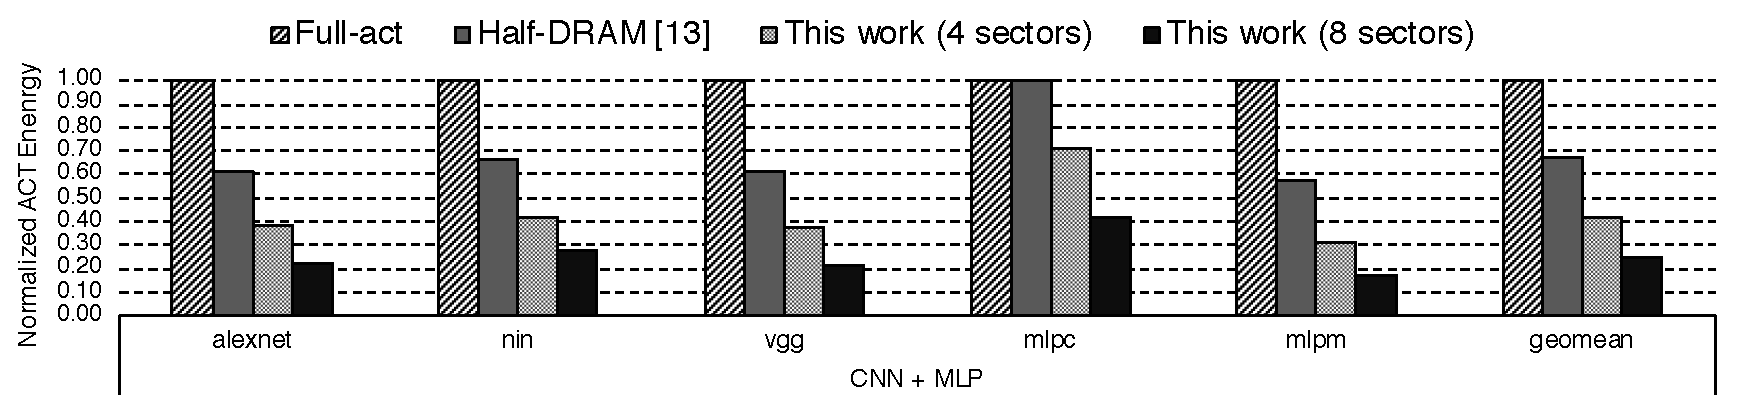
\includegraphics[width=\linewidth, page=1]{figure/thesis-eval.pdf}
\caption{Activation energy savings on CNN and MLP workloads}
\label{fig:ch4:act_e_cnn}
\end{figure}

\begin{figure}[t]
    \centering
		\includegraphics[width=\linewidth, page=2]{figure/thesis-eval.pdf}
    \caption{Activation energy savings on general workloads (Rodinia and STREAM)}
    \label{fig:ch4:act_e_gen}
\end{figure}

Occasionally, the activation energy savings are affected by row buffer access patterns. For instance, memory accesses in mlpc frequently fall on both halves of a row buffer. This leads to little activation energy savings with the Half-DRAM configuration. Figure~\ref{fig:ch4:DRAM_e_cnn} and \ref{fig:ch4:DRAM_e_gen} show how the activation energy savings are translated to DRAM-wide energy savings. The {\it 8-sector} configuration achieves 7.6\% energy savings on average with maximum savings of 14.1\%.

\begin{figure}[t]
    \centering
        \includegraphics[width=\linewidth, page=3]{figure/thesis-eval.pdf}
    \caption{DRAM energy savings on CNN and MLP workloads}
    \label{fig:ch4:DRAM_e_cnn}
\end{figure}

\begin{figure}[t]
    \centering
        \includegraphics[width=\linewidth, page=4]{figure/thesis-eval.pdf}
    \caption{DRAM energy savings on general workloads (Rodinia and STREAM)}
    \label{fig:ch4:DRAM_e_gen}
\end{figure}

\section{Performance Impact}
%Workload characteristics
Figure~\ref{fig:ch4:perf_cnn} demonstrates that both CNN and MLP workloads are tolerant of increased memory latency. The CNN workloads are known to compute-intensive as convolution layers, which dominates the execution time of a CNN, have a lot of data reuse~\mycite{jouppi2017tpu} to have relatively low off-chip memory access rate. Thus, they are able to maintain a high degree of memory-level parallelism and hence IPC. In contrast, MLP workloads, which are composed of fully-connected layers only, are known to be memory-intensive as there is no reuse of weight parameters in these layers. However, compared with recent results from Google's TPU~\mycite{jouppi2017tpu}, our MLP workloads are less memory-intensive due to fewer layers and smaller input data sets (Cifar-10 and MNIST). MLP workloads also have a lot of memory-level parallelism and is not sensitive to memory latency. Overall, both CNN and MLP workloads show only negligible IPC degradation.

\begin{figure}[t]
    \centering
        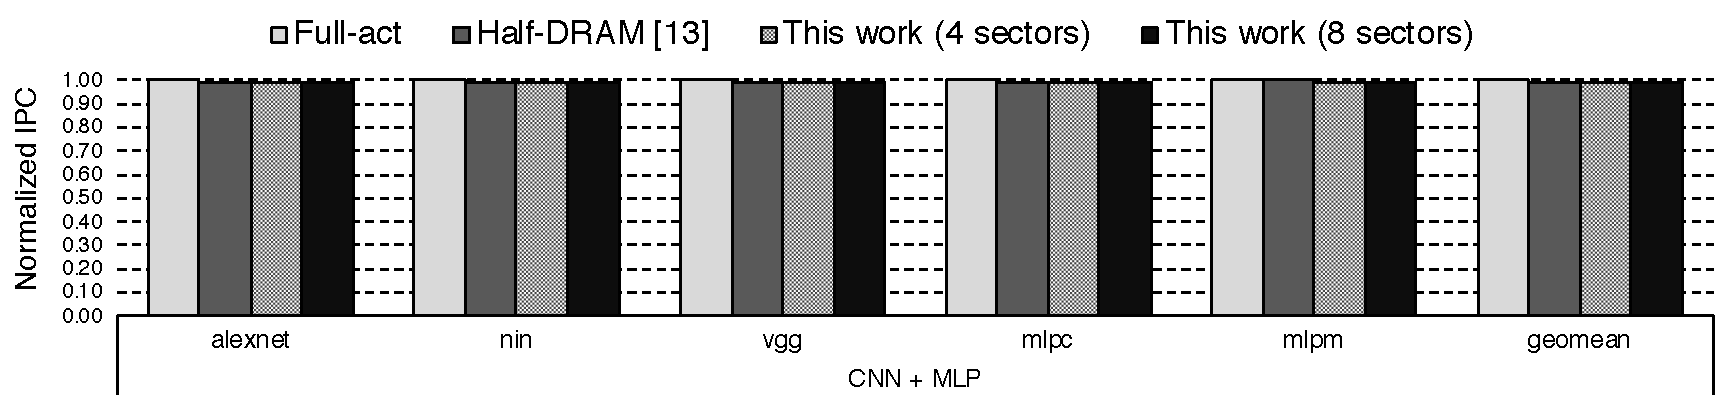
\includegraphics[width=\linewidth]{figure/perf-1.pdf}
    \caption{Performance degradation on CNN and MLP workloads}
    \label{fig:ch4:perf_cnn}
\end{figure}

\begin{figure}[t]
    \centering
        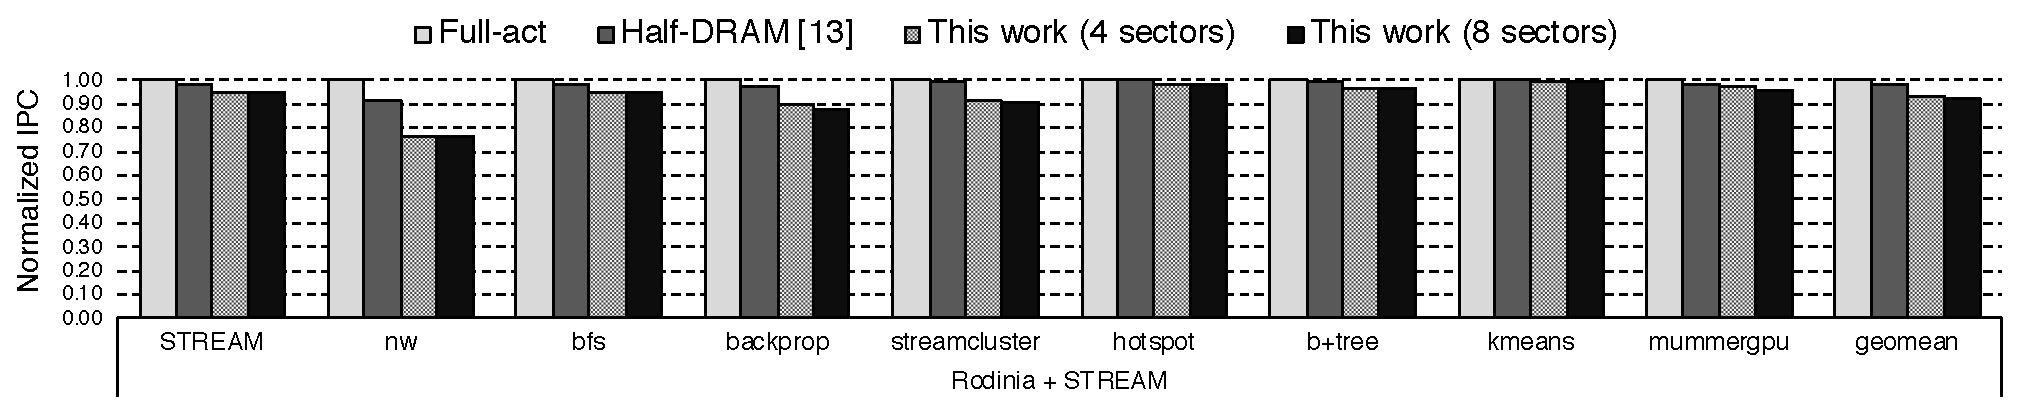
\includegraphics[width=\linewidth]{figure/perf-2.pdf}
    \caption{Performance degradation on general workloads (Rodinia and STREAM)}
    \label{fig:ch4:perf_gen}
\end{figure}

%Rodinia characteristics
To evaluate performance impact on non-DNN workloads we take memory-intensive GPU workloads from Rodinia~\mycite{rodinia} as shown on Figure~\ref{fig:ch4:perf_gen}. These workloads have a lower degree of memory-level parallelism than DNN workloads. For instance, needleman-wunsch (nw) has a fairly complex control flow with frequent branch divergence, thus suffering up to 22\% IPC degradation with the proposed scheme. In contrast, other workloads, such as hotspot, kmeans, and streamcluster, are compute-intensive with a high degree of memory-level parallelism, thus experiencing less performance hit than the others.


%Bank structure latency overhead
The IPC degradation is attributed to a couple of reasons. First, due to the narrower datapath between a DRAM mat and the I/O, the column access time (\texttt{tAA}) is increased substantially. This also negatively affects the latency of a column read/write request directed to the same bank as the previous column request. Second, there is an additional latency cost (8ns in our setup) when a new {\it sector} needs to be activated in the currently open row. Our proposed DRAM device activates the requested {\it sector} lazily only when a column request is directed to it. By activating only those {\it sectors} that are actually read or written, we may have a performance hit for workloads with good spatial locality in DRAM accesses. This problem may be alleviated by increasing the {\it sector} granularity (e.g., from 8 {\it sectors} to 4 {\it sectors} per DRAM row), while losing some of the energy savings with potential overfetching within a {\it sector}.

\section{Area Overhead}
We estimated area overhead incurred by additional circuitry using CACTI-3DD~\mycite{cacti3dd}.
The area overhead for the portion added to the inside of the dram core includes the following:
latches which hold valid bit vector per bank, and 9 AND gates added per subarray.
The \textit{sector} selection latch logic is modeled based on the local sense amplifier inside the core, 
and the NAND gate uses the NAND gate model used in the core.
Overall, the die area overhead is 0.3\% which we believe acceptable.


\chapter{Conclusion}
This thesis presents a practical partial activation scheme for 3D stacked DRAM with applications to deep learning workloads without significant modifications to the standard HBM2 DRAM interface. To achieve high energy efficiency while maintaining low performance overhead, we exploit the latency tolerance of emerging deep learning workloads to trade DRAM latency for energy efficiency. Consequently, our proposal demonstrates substantial DRAM energy savings with minimal performance hit for both the deep learning workloads and other conventional GPU workloads. This benefit comes with a very low implementation (area) cost and minimal adjustments of DRAM timing parameters over the standard HBM2 DRAM interface.


\clearpage
%\section{Table insertion}
%\subsection{Basic}
%\url{https://www.tablesgenerator.com/latex_tables} creates the most basic template!
%
%\clearpage
%\subsection{Advanced}
%The most annoying part of latex work is table insertion.
%Size modification, highlights, and annotation in table are very annoying compared to Hancom, so many people turn to it.
%However, latex will feel much easier if you learn only the following introductions for graduation thesis.
%
%\textit{adjustbox}: It adjusts the overall size of the table. If not, a table may be generated  beyond the document scope.
%
%\textit{columncolor}: It shades the entire column to emphasize the results of my model.
%
%\textit{footnotemark and footnotetext}: Inside the table, the $\setminus$footnote does not work. 
%For this reason, footnotemark and footnotetext are used.
%Note that the page on which the annotation exists is not always the same (...) as the table.
%When the footnotemark is used several times inside the table, the annotation number becomes strange.
%In this case, use \textit{addtocounter}.
%\newline
%\newline
%If you need more than this, let's do googling.

\clearpage

%\addtocounter{footnote}{-1}
%\footnotetext{For a fair comparison, we report EntNet's result~\mycite{henaff2016tracking} which was jointly trained on all tasks. It was written in the appendix of the paper.}
%\addtocounter{footnote}{+1}
%\footnotetext{Our implementation. The result is different from what \myauthor{santoro2017simple} mentioned, which is caused by the initialization~\mycite{santoro2017simple}.}
%

%\chapter{Reference insertion}
%\section{Insert reference right before the period mark}
%Do not use conventional $\sim\setminus$cite\{\}.

%ex: blah blah~\cite{bishop2006}.
%Because of ( ), I defined `mycite' to appear reference number with [ ].

%ex: blah blah~\mycite{bishop2006}.


%\clearpage
%\section{Insert reference to the author name}
%Sometimes you need to put a reference to the author name. 
%To do this, I defined `myauthor'.
%ex: \myauthor{bishop2006} said blah blah~\mycite{bishop2006}.

\begin{bibpage}
	\bibliographystyle{ieeetr}
	\bibliography{references}
\end{bibpage}


\appendix
%\chapter{Appendix title 1}
%The appendix does not appear in the table of contents.
%In this case, open a .toc file (or click the table of contents page with holding ctrl) and add a line below the bibliography.
%
%\contentsline {chapter}{Bibliography}{8}{section*.9} % 현재 Bibliography
%\contentsline {chapter}{Appendix}{9}{section*.10} % {9}는 페이지 번호이므로 알아서 맞추자
%\contentsline {section}{\numberline {A}Appendix title 1}{9}{section.Alph0.1}
%\contentsline {section}{\numberline {B}Appendix title 2}{10}{section.Alph0.2}
%
%\chapter{Appendix title 2}

\keywordalt{CNN, GPU, DRAM 아키텍처, 에너지 효율, HBM2}
\begin{abstractalt}
GPU는 딥 러닝 애플리케이션을 실행하는 데 널리 사용된다.
오늘날의 high-end GPU는 HBM (High-Bandwidth Memory)과 같은 3D 적층 DRAM 기술을 채택하여 
엄청난 대역폭을 제공하므로 많은 전력을 소비한다.
GPU에서 수천 개의 동시 스레드가 발생하면 빈번한 row buffer conflict로 인해 상당한 양의 DRAM 에너지가 낭비된다.
이러한 낭비를 줄이기 위해 3D 적층 DRAM에 대한 partial row activation 기법을 제안한다.
풍부한 memory-level parallelism 이 있는 딥 러닝 워크 로드의 latency tolerance를 활용해서, DRAM latency를 지불하고 에너지 절감을 얻을 수 있다.
본 제안에서 딥 러닝 및 기타 기존 GPU 워크 로드에서 성능 저하를 최소화하면서 DRAM activation energy의 상당한 절감 효과를 보여준다.
본 제안은 매우 낮은 면적 비용으로 표준 HBM2 DRAM 인터페이스에 대한 DRAM 타이밍의 최소한의 변경만으로 구현할 수 있다는 장점이 있다.
\end{abstractalt}

\acknowledgement
먼저 제가 학업을 수행할 수 있도록 다방면으로 지원을 아끼지 않으신 존경 하는 부모님 감사드립니다.
부모님이 아니었다면 제가 하는 어떠한 일도 이루어질 수 없었을 것 입니다.
저의 학문과 연구의 길을 밝혀주신 등대와 같은 교수님 존경하고 감사합니다.
항상 저에게 따끔한 조언 뿐만 아니라 긍정적인 에너지와 계속 연구 할 수 있는 힘을 주셨습니다.

연구실에서 3년이라는 시간동안 동고동락해온 찬노형과 기태형 그리고 성민이형 으로 구성된 
Typed Architecture team과 함께 연구 하면서 많은 것들을 배웠고 
그 결과물들을 학회에 제출 할 수 있어서 뜻 깊은 경험이었습니다.

본 연구를 하면서 도움을 주신 분들께 감사를 드립니다.
연구의 디테일 한 부분까지 검토 해주신 함태준 박사님,
학부 인턴임에도 연구에 많은 기여를 한 한성이에게 깊은 감사를 전합니다.

연구실 생활을 하면서 많은 긍정적인 에너지를 공유할 수 있어서 정말 감사했습니다.
힘들때 술 한잔 기울일 수 있었던 학범이형과 재영이형, 무슨얘기를 하더라도 잘 웃어주고 들어주는 영환이형,
가끔 연구에 지쳤을때, 보드게임을 함께 즐겼던 준이형과 문경이 누나,
뭐든지 물어봐도 거의 모르는게 없는 종현이형,
2년동안 같이 수업도 듣고 연구실 생활의 시작과 끝을 함께한 대연이와 천이,
수학도 잘하고 논리의 끝이 날카로운 성학이,
힘들 때마다 “이겨내야죠” 라고 말해줬던 예진이, 타르트와 쿠키를 잘 만들어왔던 성준이,
회사생활을 함에 있어서 현실적이고 실질적인 조언을 많이 해주신 신이형 석용이형,
행정 업무를 맡아 주시고 발레를 좋아하는 미림누나
연구실 모든 분들 감사드립니다.
마지막으로, 이 논문이 나오는 데 간접적이나마 도움이 된 분들 모두 감사드립니다.
2019년 1월

%Thanks!

\end{document}
